\let\negmedspace\undefined
\let\negthickspace\undefined
\documentclass[journal]{IEEEtran}
\usepackage[a5paper, margin=10mm, onecolumn]{geometry}
%\usepackage{lmodern} % Ensure lmodern is loaded for pdflatex
\usepackage{tfrupee} % Include tfrupee package

\setlength{\headheight}{1cm} % Set the height of the header box
\setlength{\headsep}{0mm}     % Set the distance between the header box and the top of the text

\usepackage{gvv-book}
\usepackage{gvv}
\usepackage{cite}
\usepackage{amsmath,amssymb,amsfonts,amsthm}
\usepackage{algorithmic}
\usepackage{graphicx}
\usepackage{textcomp}
\usepackage{xcolor}
\usepackage{txfonts}
\usepackage{listings}
\usepackage{enumitem}
\usepackage{mathtools}
\usepackage{gensymb}
\usepackage{comment}
\usepackage[breaklinks=true]{hyperref}
\usepackage{tkz-euclide} 
\usepackage{listings}
\usepackage{gvv}                                        
\def\inputGnumericTable{}                                 
\usepackage[latin1]{inputenc}                                
\usepackage{color}                                            
\usepackage{array}                                            
\usepackage{longtable}                                       
\usepackage{calc}                                             
\usepackage{multirow}                                         
\usepackage{hhline}                                           
\usepackage{ifthen}                                           
\usepackage{lscape}
\begin{document}

\bibliographystyle{IEEEtran}
\vspace{3cm}

\title{9.5.3}
\author{AI24BTECH11024-Pappuri Prahladha}
% \bigskip
{\let\newpage\relax\maketitle}

\renewcommand{\thefigure}{\theenumi}
\renewcommand{\thetable}{\theenumi}
\setlength{\intextsep}{10pt} % Space between text and floats


\numberwithin{equation}{enumi}
\numberwithin{figure}{enumi}
\renewcommand{\thetable}{\theenumi}


\textbf{Question:}\\
The cartesian equation of a line $AB$ is $\frac{2x-1}{12}=\frac{y+2}{2}=\frac{z-3}{3}$.Find the direction cosines of a line parallel to line $AB$.
\\
\textbf{Solution: }\\
\begin{table}[h!]
    \renewcommand{\thetable}{1}
    \centering
    \begin{tabular}[12ptx]{ |c| c|}
\hline\textbf{Term} & \textbf{Description}\\
\hline
$m$&Direction vector of line \\
\hline
\end{tabular}

    \caption{Terms used}
    \label{TABLE 1:}
\end{table}\\
The direction vector of the given line is$\colon$
\begin{equation*}
    \vec{m}=\begin{pmatrix}
        6\\
        2\\
        3
    \end{pmatrix}
\end{equation*}
The unit vector of a line having direction vector $m$ is given by $\colon$
\begin{equation}
    \frac{m}{||m||}
\end{equation}
The direction cosines are elements of above vector  \\
From 0.1 the unit vector along $AB$ is$\colon$\\
\begin{equation}
\frac{1}{\sqrt{49}}\begin{pmatrix}
    6\\
    2\\
    3
\end{pmatrix}
\end{equation}
$\therefore$ the direction cosines of line parallel to line$AB$ are the elements of above vector.
 \begin{figure}[h!]
   \centering
   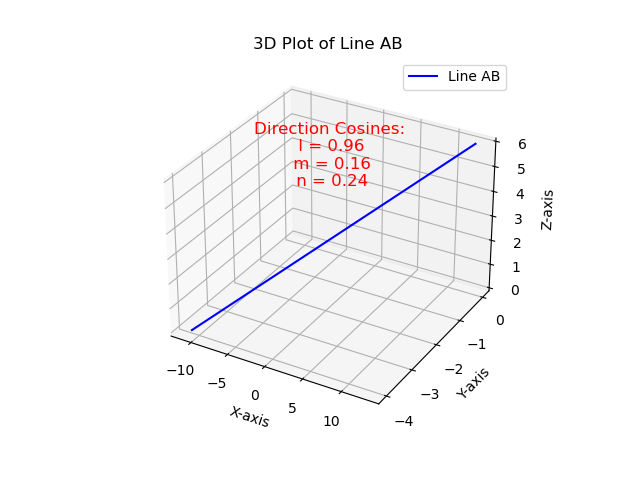
\includegraphics[width=0.7\linewidth]{figs/figure1.png}
   \caption{Plot showing the line $AB$}
   \label{stemplot}
\end{figure}
\end{document}

